\documentclass[10pt,letterpaper]{article}
\usepackage[T1]{fontenc}
\usepackage[utf8]{inputenc}
\usepackage[sc]{mathpazo}
\usepackage[margin=.72in,headheight=14pt]{geometry}
\usepackage{microtype,graphicx,booktabs,array,amsmath,xcolor,fancyhdr,enumitem,xurl,hyperref}
\definecolor{Ink}{HTML}{102A43}
\definecolor{Teal}{HTML}{087F8C}
\definecolor{Gold}{HTML}{D69A2D}
\definecolor{Red}{HTML}{B94046}
\definecolor{Pale}{HTML}{EDF4F6}
\hypersetup{colorlinks=true,urlcolor=Teal,linkcolor=Teal,pdftitle={The Possibility Engine: Executive Brief},pdfauthor={Vincent Boucher}}
\urlstyle{same}
\color{Ink}
\setlength{\parindent}{0pt}\setlength{\parskip}{5pt}
\setlength{\emergencystretch}{2em}
\setlength{\tabcolsep}{5pt}\renewcommand{\arraystretch}{1.13}
\setlist{nosep,leftmargin=1.3em}
\pagestyle{fancy}\fancyhf{}
\fancyhead[L]{\small\textsc{AGI Alpha Flywheel}}
\fancyhead[R]{\small\textsc{Executive Brief / 28 October 2026}}
\fancyfoot[L]{\footnotesize Vincent Boucher \enspace / \enspace President of MONTREAL.AI}
\fancyfoot[R]{\small\thepage\,/\,2}
\newcolumntype{L}[1]{>{\raggedright\arraybackslash}p{#1}}
\newcommand{\briefhead}[1]{\vspace{7pt}{\large\bfseries\color{Teal}#1}\par}
\begin{document}
{\fontsize{30}{33}\selectfont\bfseries THE POSSIBILITY ENGINE}\par
{\large Construct the means. Test the economy. Earn the next step.}\par
\vspace{7pt}
\colorbox{Pale}{\parbox{.96\textwidth}{\textbf{Decision: STOP standalone expansion.} A working construction and successor passed digital acceptance. The commercial candidate failed complete-cost testing; no replacement earned flagship status in the reopened search.}}

\briefhead{What was built}
\textbf{EventWeaver} turns a precise temporal event contract into a functional firmware design pack: executable models, C++ and Verilog, replayable traces and independent acceptance checks. It supports independent groups, overlapping anchors and a veto that can cancel a completed event sequence through its decision deadline. The successor adds a new grammar: one accepted decision becomes a virtual input to another stage.

The beneficiary is a small instrument OEM or experimental photonics team with an existing digitized event interface. The first deliverable is bounded digital logic. A calibrated clock, physical board interface, timing closure and demonstrated experiment benefit remain separate gates. The use case is an application hypothesis, not a recovered customer request.

\begin{center}
\begin{tabular}{L{.29\textwidth}L{.29\textwidth}L{.29\textwidth}}
\toprule
{\Large\color{Teal}\textbf{768 / 768}} & {\Large\color{Teal}\textbf{48 / 48}} & {\Large\color{Teal}\textbf{40}}\\
Fresh main traces passed across 24 specifications & Fresh successor traces passed across six networks & Bounded equivalence checks passed, with explicit proof depths\\
\bottomrule
\end{tabular}
\end{center}

\briefhead{The first experience}
The buyer declares channels, time windows, deadline and reset semantics in JSON. The system rejects unsupported requests, generates a kernel and replays the agreed trace. Acceptance requires exact outputs under the unchanged contract. A failure produces a counterexample, a refusal or a bounded correction. The offline browser edition lets the reader toggle late veto and reset and inspect the resulting decisions.

\begin{center}
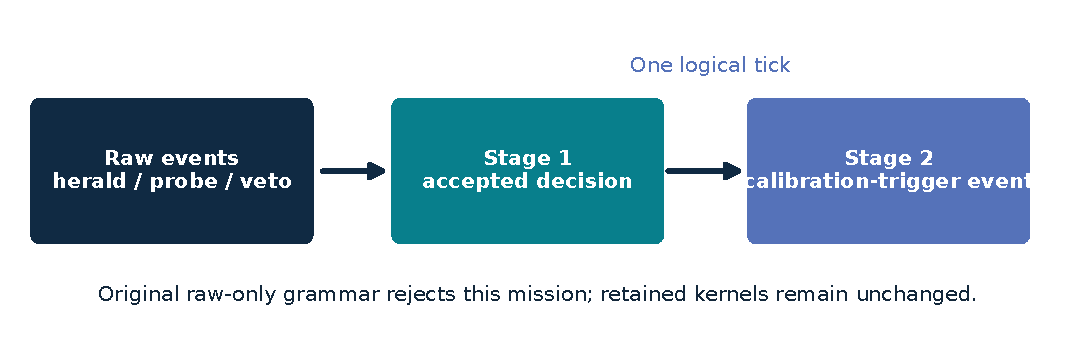
\includegraphics[width=.91\textwidth]{figures/successor_network.pdf}
\end{center}

\briefhead{What the controls changed}
A separately authored, current-AI-assisted conventional implementation \textbf{tied on functional acceptance}. An ordinary library containing the same retained artifact \textbf{tied on succession}. The EventWeaver Python model was about \textbf{45 times slower} than the conventional model on the fresh workload; paired RTL replay is not a hardware-speed comparison.

Six predeclared removal fixtures distinguish necessary semantics from a necessary implementation. Removing delayed veto or group isolation creates false decisions; removing the virtual link loses the successor outcome. Replacing our compiler with conventional RTL preserves all six outcomes. This supports useful construction, not exclusive novelty or proven new commercial feasibility.

{\footnotesize\color{Ink}\textbf{Scope.} Construction, compilation, replay, synthesis and checks were executed. Buyers, contracts, labor, payments, demand and financing were simulated. All monetary results are conditional modeled 2026 US dollars. No purchases, outreach or live financial actions occurred.}
\newpage
\briefhead{The commercial loop failed before reinvestment}
Development compared 15 price--arrangement policies: bespoke work, three-order pooling and supported-library service at five prices. All lost money. The least-loss policy, supported-library service at a posted \textbf{US\$1,200}, was frozen for fresh confirmation, not authorized for launch. Buyers could choose rivals, internal teams using current AI, free tools, waiting or doing nothing.

\begin{center}
\begin{tabular}{L{.64\textwidth}r}
\toprule
\textbf{Fresh base case: 1,024 histories} & \textbf{Mean or stated quantile}\\
\midrule
Accepted initial design packs & 7.94\\
Net recognized revenue / net customer cash & US\$9,024 / US\$8,836\\
Complete project cost & US\$38,653\\
Operating contribution before fixed costs & US\$\(-3,928\)\\
\textbf{Full-project profit / return on cost} & \textbf{US\$\(-29,628\) / \(-76.7\%\)}\\
Loss frequency under the base model & 1,024 / 1,024\\
95th percentile unrestricted capital required & US\$36,496\\
Variable service hours per accepted pack & 9.17\\
\bottomrule
\end{tabular}
\end{center}

Costs include discovery, failed work, construction, verification, inference, sales, support, correction, refunds, maintenance and financing. The US\$4,100 successor/retention option is charged once. Refundable deposits remain restricted until acceptance. The base cash requirement fits the modeled US\$45,000 equity. Seven stress histories retain terminal debt; later interest and creditor recovery are outside the model. Renewals assume acceptance/full collection after procurement, without a second failure, warranty or default cycle.

Independent reconstruction checked \textbf{10,240 histories, 1,265,250 journal entries} and the buyer/seller decisions. Nine additional scenarios also lost in every history. Higher demand, competitor responses, an identical free library and cheaper AI for all firms failed to rescue the policy. The finite strategic game selected no entry when exit was permitted.

\textbf{The scale hurdle is concrete.} A constant-mix calculation needs 82 accepted packs to break even; reserved 180-day capacity is about 42. At unchanged demand, negotiated price would need to rise from roughly US\$1,153 to US\$4,883, while the tested demand response already collapses at lower fees. Neither 100\% acceptance nor zero direct delivery cost closes the full bill. The billion-dollar ambition is unearned.

\briefhead{A decision that reopens the search}
EventWeaver is retained as a tested construction and rejected commercial candidate. The campaign reopened discovery after that rejection, examining recent world-model/robotics, material-realization and cross-owner scientific-experiment openings. No replacement had both an exercised essential construction and a defensible commercial bridge within the bounded campaign.

The strongest new opening is a \textbf{counterfactual experience foundry}: create rare but physically calibrated interactions and deliver a robot recovery skill that improves held-out real outcomes. Recent model releases make the investigation timely; generated video or simulator success alone would not establish physical transfer. The next decisive gate is a matched, bounded transfer experiment against competent conventional simulation and current AI, with a named operational beneficiary and measured outside cost. This is a new research opening, not a delivered product.

\briefhead{What the edition leaves behind}
The complete paper, source, browser reader, runnable compiler and successor, conventional controls, frozen protocols, full histories, economic scenarios, independent audits, preserved failures and developer handoff form one reproducible review package. The final decision is \textbf{stop this standalone launch; preserve the instrument; admit a new flagship only after its productive and commercial bridge earns selection}. Canonical repository publication remains subject to the existing owner's full-source qualification; LinkedIn text remains an unposted draft.

{\footnotesize\textbf{Evidence guide.} See the full paper, Sections 2--5 and 8--12; \path{results/technical_confirmation/summary.json}, \path{results/business_confirmation.json}, \path{audit/accounting_confirmation.json} and \path{research/return_to_search.json}. Sampling precision is conditional on the model and does not resolve unknown real-world demand.}
\end{document}
